\chapter{Planification du projet}
\addcontentsline{toc}{chapter}{Chapitre 2 : Planification du projet}

 

 \addcontentsline{toc}{section}{Introduction} % Ajoute "Introduction" dans la table des matières

\section*{Introduction}
Dans ce chapitre, nous allons en premier lieu définir les acteurs en détaillant les besoins fonctionnels et non fonctionnels de notre application. En second lieu, nous allons présenter l’architecture de notre plateforme.
% Numérotation

\renewcommand{\thesection}{\Roman{section}.} 
\renewcommand{\thesubsection}{\arabic{subsection}.}
\renewcommand{\thesubsubsection}{\thesubsection\arabic{subsubsection}}
% Section 1

\section{Spécification des besoins}


\subsection{Besoins fonctionnels}
Notre application permet à Administrateur :
\begin{itemize}
    \item Gérer les utilisateurs.
    \item Gérer les événements.
    \item Gérer les catégories.
    \item Consulter les statistiques.
\end{itemize}

Notre application permet à Gestionnaire des événements :
\begin{itemize}
    \item Créer un compte.
    \item Mettre à jour son profil.
    \item Gérer les événements.
    \item Gérer les inscriptions.
    \item Envoyer des rappels.
    \item Accéder aux statistiques des événements.
\end{itemize}

Notre application permet à Utilisateur :
\begin{itemize}
    \item Créer un compte.
    \item Mettre à jour son profil.
    \item Lister les événements.
    \item S’inscrire à un événement.
    \item Envoyer des messages pour demande d'information.
    \item Faire un commentaire.
\end{itemize}

\subsection{Besoins non fonctionnels}

\subsubsection*{Performance:}
\begin{itemize}
    \item La plateforme doit supporter jusqu’à 500 utilisateurs simultanés sans dégrader les performances.
\end{itemize}

\subsubsection*{Sécurité:}
\begin{itemize}
    \item Les mots de passe doivent être cryptés pour garantir leur sécurité.
    \item Des règles strictes d’accès aux données doivent être définies selon les rôles.
    \item La plateforme doit être protégée contre les attaques comme les injections SQL et XSS.
\end{itemize}

\subsubsection*{Fiabilité:}
\begin{itemize}
    \item La plateforme doit être disponible 99,9\% du temps avec un minimum de temps d’arrêt.
    \item Les données doivent être sauvegardées quotidiennement pour éviter leur perte.
\end{itemize}

\subsubsection*{Scalabilité:}
\begin{itemize}
    \item L’architecture doit évoluer pour supporter une augmentation d’utilisateurs et d’événements.
    \item Il doit être facile d'ajouter de nouvelles fonctionnalités à la plateforme.
\end{itemize}

\subsubsection*{Accessibilité:}
\begin{itemize}
    \item La plateforme doit respecter les normes d’accessibilité (WCAG 2.1).
    \item Elle doit être compatible avec les lecteurs d’écran et utiliser des couleurs contrastées.
\end{itemize}

\subsubsection*{Maintenabilité:}
\begin{itemize}
    \item Le code doit être bien structuré, documenté et facile à modifier.
    \item Des tests automatisés doivent être utilisés pour détecter rapidement les erreurs.
\end{itemize}

\subsubsection*{Portabilité:}
\begin{itemize}
    \item La plateforme doit être compatible avec les navigateurs principaux (Chrome, Firefox, Edge, Safari).
    \item L’hébergement doit se faire sur des serveurs cloud (AWS, Azure).
\end{itemize}

% Section 2
\section{Gestion de projet avec Scrum}

\subsection{Équipe SCRUM et rôles}
SCRUM définit trois rôles, comme reflété dans la figure ci-dessous :\\
— Product Owner : Mr. Yasser Ben Ali\\
— Scrum Master : Mme. Hella Jebali\\
— L’équipe de développement : Wided Laabidi et Mohamed Aziz Barrouta

\begin{figure}[H]
    \centering
    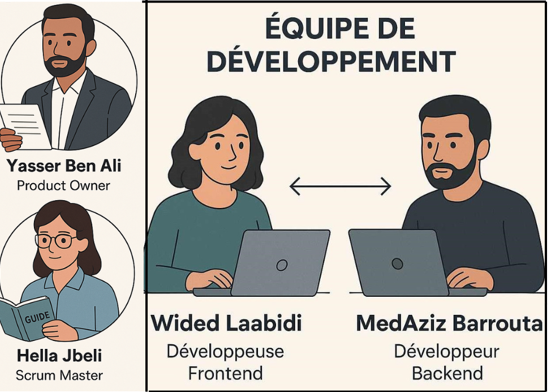
\includegraphics[width=0.7\linewidth]{projet/images/equipeScrum.png}
    \caption{L'équipe Scrum}
    \label{fig:equipe_scrum}
\end{figure}

\subsection{Product Backlog}
C'est le composant le plus basique dans le processus Scrum. Nous l’avons utilisé pour
Planifier la réalisation de chaque sprint. Donc, il contient des fonctionnalités
requises pour la construction d’un produit, ainsi que tous les éléments nécessitant
L’intervention de l’équipe. Ces éléments sont classés par ordre de priorité et de
Leur dépendance, ce qui permet de spécifier l’ordre de leur réalisation.\\


\begin{table}[h!]
\renewcommand{\arraystretch}{1.6}
\setlength{\tabcolsep}{5pt}
\centering
\begin{tabular}{|c|c|m{7cm}|c|c|}
\hline
\textbf{ID} & \textbf{Sprint} & \textbf{User Story} & \textbf{Priorité} & \textbf{Complexité} \\
\hline


\multirow{3}{*}{2} & \multirow{3}{*}{\parbox{3cm}{\centering Authentification\\ et gestion des utilisateurs}} 
& En tant qu’utilisateur , je veux m’inscrire et me connecter pour accéder à mon espace.. & Élevé & Moyenne \\
\cline{3-5}
&& En tant que gestionnaire , je veux m’inscrire et me connecter pour accéder à mon espace.. & Élevé & Moyenne \\
\cline{3-5}
& & En tant qu’administrateur, je veux gérer les rôles des utilisateurs pour contrôler l’accès.. & Élevé & Moyenne \\
\cline{3-5}
\hline


\multirow{7}{*}{3} & \multirow{7}{*}{\parbox{3cm}{\centering Gestion\\ des évenements }} 
& En tant qu’administrateur, je veux  modifier  des événements. & Élevé & Moyenne \\
\cline{3-5}
& & En tant qu’administrateur, je veux supprimer des événements. & Élevé & Moyenne \\
\cline{3-5}
& & En tant qu’administrateur, je veux Consulter des événements. & Élevé & Moyenne \\
\cline{3-5}
& & En tant qu’administrateur, je veux Approver des événements. & Élevé & Moyenne \\
\cline{3-5}
& & En tant que Gestionnaire , je veux Créer des événements. & Élevé & Moyenne \\
\cline{3-5}
& & En tant que Gestionnaire, je veux Modifier des événements. & Élevé & Moyenne \\
\cline{3-5}
& & En tant que Gestionnaire, je veux Supprimer  des événements. & Élevé & Moyenne \\
\hline

\multirow{3}{*}{4} & \multirow{3}{*}{\parbox{3cm}{\centering  Inscription et\\  interaction utilisateur }} 
& qu’utilisateur, je veux m’inscrire à un événement. & Élevé & Moyenne \\
\cline{3-5}
& & En tant qu’utilisateur, je veux recevoir une notification après inscription. & Élevé & Moyenne \\
\cline{3-5}
& & En tant qu’utilisateur, je veux laisser un feedback après participation. & Élevé & Moyenne \\

\hline
\multirow{3}{*}{5} & \multirow{3}{*}{\parbox{3cm}{\centering Gestion avancée \\et tableaux de bord }} 
& En tant qu’utilisateur, je consulte les statistique globales & Haute  & Moyenne \\
\cline{3-5}
& & En tant que Geestionnaire j'accéder au statistique des évenement  & Élevé & Moyenne \\
\cline{3-5}
\hline
\end{tabular}
\caption{Product Backlog}
\end{table}

\clearpage
\subsection{Planification de sprint}
La préparation des sprints revêt une importance capitale dans la concrétisation des projets
SCRUM. Nous diviserons notre projet en 4 releases qui seront constituées de 6 sprints. La figure
suivante illustre la division des releases en sprints.
\begin{figure}[H]
    \centering
    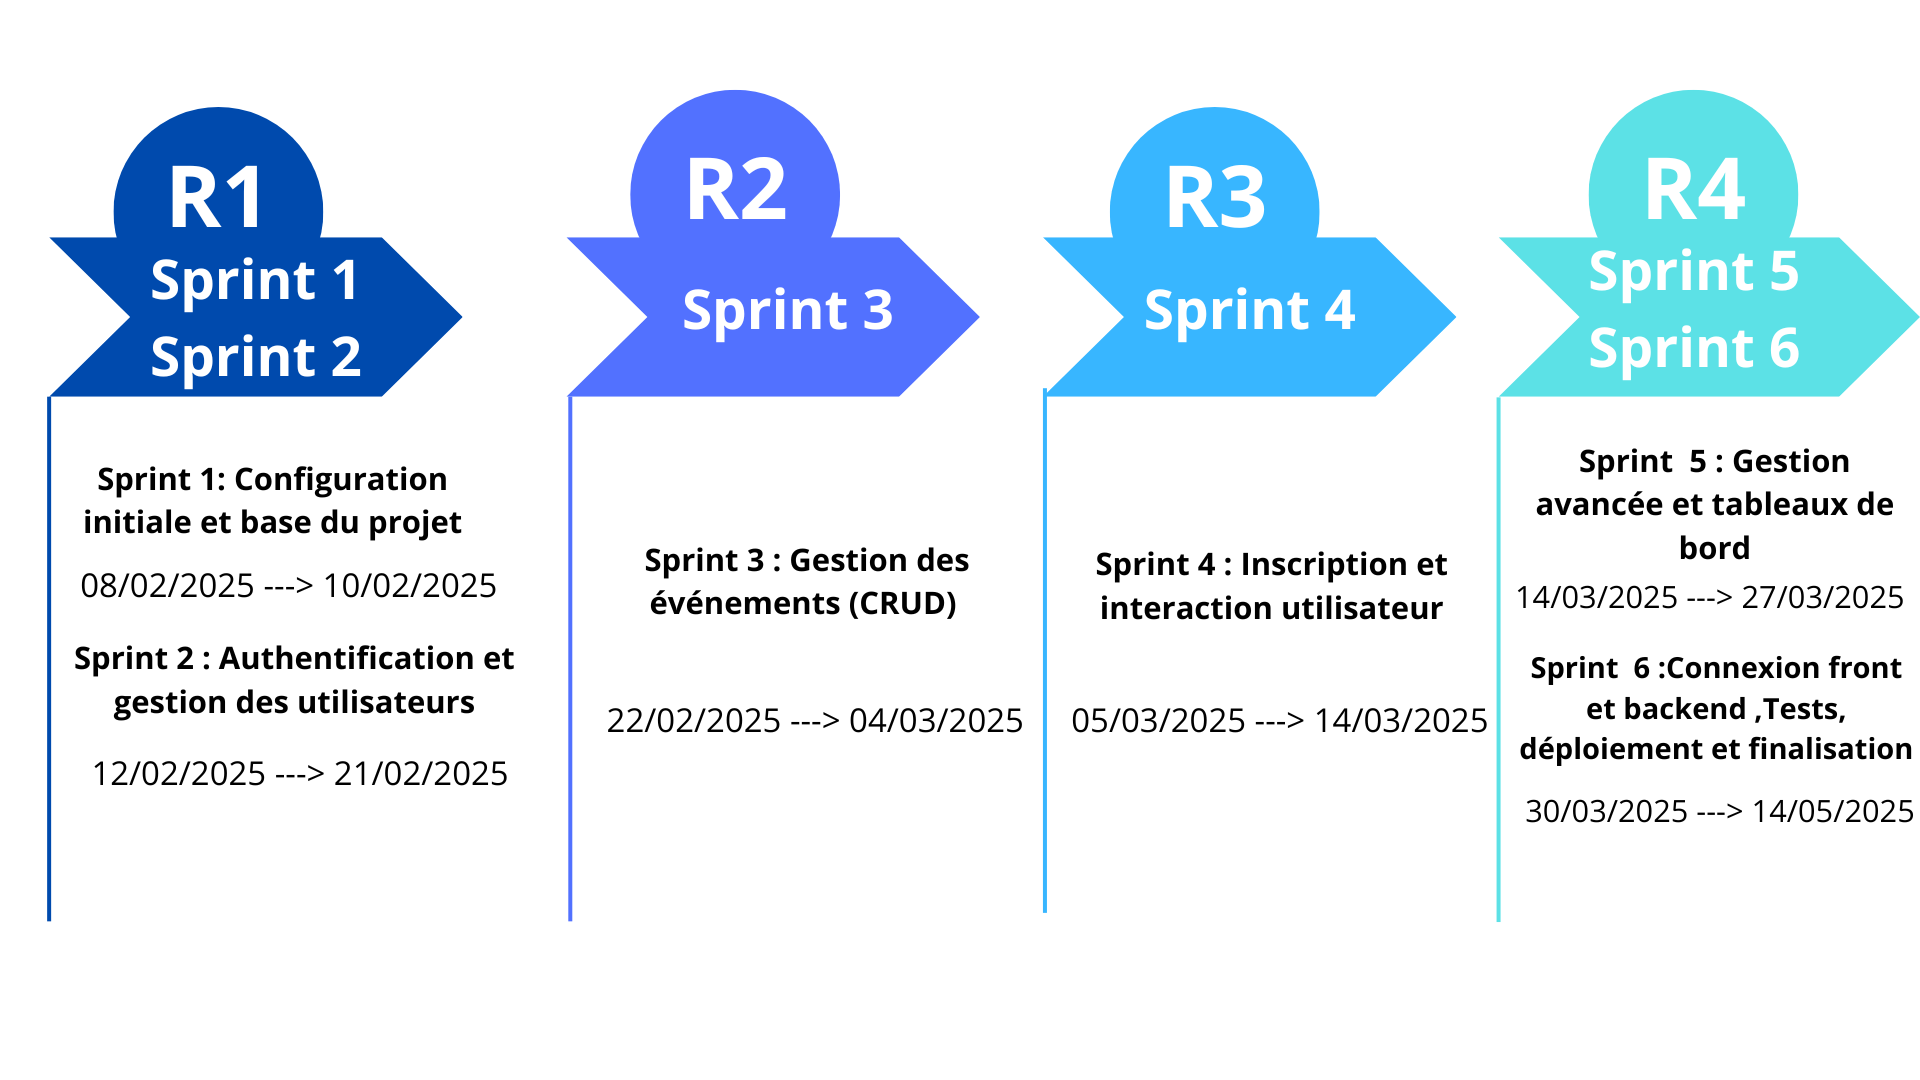
\includegraphics[width=0.9\linewidth]{projet/images/R1.png}
    \caption{Planification des sprints}
    \label{fig:equipe_scrum}
 \end{figure}

% Section 3
\section{Diagrammes de cas d'utilisations général}

\subsection{Identification des acteurs}

Dans cette section, nous définissons les acteurs du système ainsi que leurs rôles respectifs. Le tableau~\ref{tab:identification_acteurs} ci-dessous récapitule ces informations.

\begin{longtable}{|p{4cm}|p{5cm}|p{6cm}|}
\hline
\textbf{Acteur} & \textbf{Rôle} & \textbf{Fonctionnalités/Services} \\ 
\hline
\parbox[c][3.5cm][c]{\linewidth}{\centering
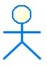
\includegraphics[width=0.3\linewidth]{projet/images/acteur.jpg} \\[0.2cm] \textbf{Administrateur}
} & 
Gérer et administrer la plateforme & 
\begin{itemize}[leftmargin=0.5cm]
    \item Gérer les utilisateurs.
    \item Gérer les événements.
    \item Consulter les statistiques.
\end{itemize} \\ 
\hline

\parbox[c][3.5cm][c]{\linewidth}{\centering
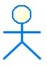
\includegraphics[width=0.3\linewidth]{projet/images/acteur.jpg} \\[0.2cm] \textbf{Utilisateur}
} & 
Participer aux événements & 
\begin{itemize}[leftmargin=0.5cm]
    \item S’inscrire aux événements.
    \item Envoyer des messages.
    \item Poster des commentaires.
\end{itemize} \\ 
\hline

\parbox[c][3.5cm][c]{\linewidth}{\centering
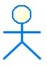
\includegraphics[width=0.3\linewidth]{projet/images/acteur.jpg} \\[0.2cm] \textbf{Gestionnaire des événements}
} & 
Organiser et gérer les événements & 
\begin{itemize}[leftmargin=0.5cm]
    \item Créer et modifier des événements.
    \item Gérer les inscriptions.
    \item Suivre les statistiques des événements.
\end{itemize} \\ 
\hline
\caption{Identification des acteurs et de leurs fonctionnalités}
\label{tab:identification_acteurs}
\end{longtable}

% Section 4

\subsection{Diagramme de contexte statique}
Ce diagramme UML montre la relation des différents acteurs avec le système.

\begin{figure}[H]
    \centering
    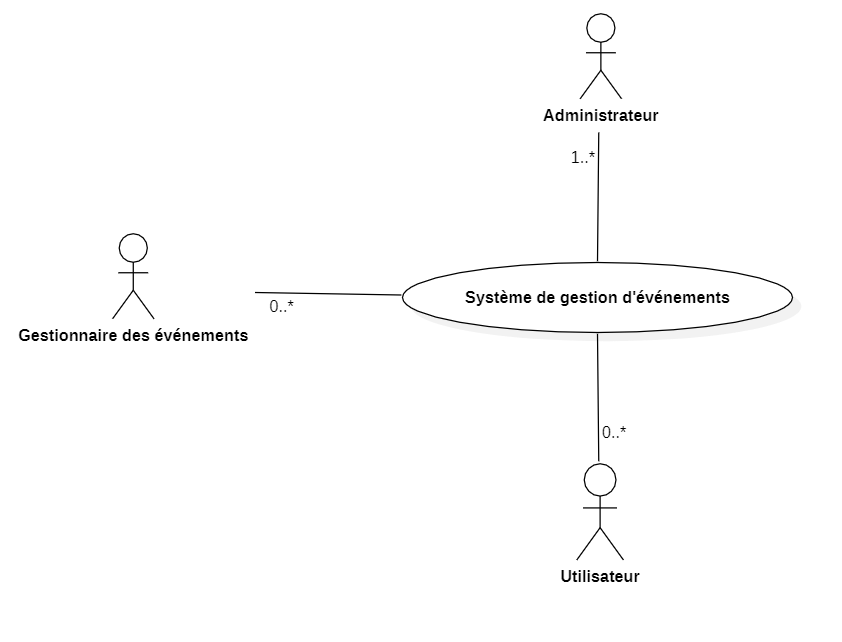
\includegraphics[scale=0.3]{projet/images/Diagramme de contexte statique.png}
    \caption{Diagramme de contexte statique}
\end{figure}

% Section 5
\subsection{Diagramme de cas d’utilisation global}
Voici le diagramme de cas d’utilisation global de notre application :

\begin{figure}[H]
    \centering
    \includegraphics[width=\textwidth]{projet/images/Diagramme de cas d’utilisation global.png}
    \caption{Diagramme de cas d'utilisation globale}
\end{figure}

\section{Diagramme de classes général}

Ce diagramme UML représente la structure de données de notre application.

\begin{figure}[H]
    \centering
    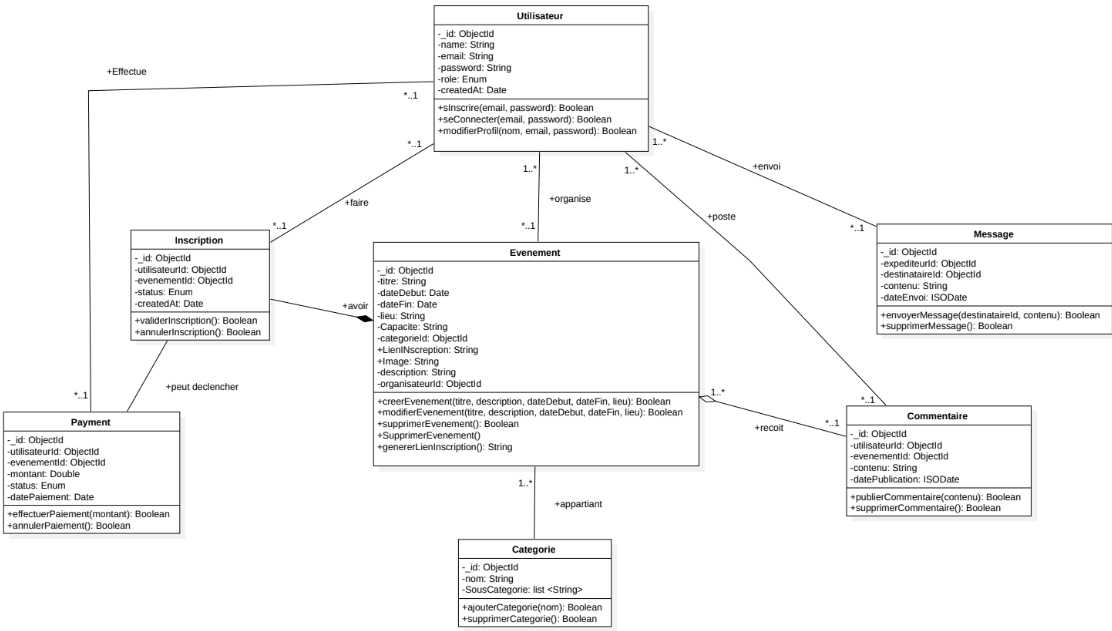
\includegraphics[width=0.95\textwidth]{projet/images/diagramme de classe.png}
    \caption{Diagramme de classes général de l'application}
    \label{fig:diagramme_classe}
\end{figure}

\section{Environnement de développement et choix techniques}

Dans cette section, nous présentons l’environnement matériel ainsi que l’environnement logiciel utilisés pour implémenter la solution informatique.

\subsection{Environnement matériel}

Nous détaillons ici les caractéristiques matérielles, notamment le processeur, la mémoire vive (RAM), le disque dur et le système d’exploitation de chaque ordinateur utilisé. Toutes les informations sont récapitulées dans le Tableau ~\ref{tab:environnement_materiel}.

\begin{table}[H]
\centering
\begin{tabular}{|l|l|l|}
\hline
\textbf{Ordinateur} & \textbf{1} & \textbf{2} \\ \hline
Propriétaire & Laabidi Wided & Barrouta Mouhamed Aziz \\ \hline
Processeur & Intel Core i5 & AMD Ryzen 5 \\ \hline
RAM & 16 Go & 8 Go \\ \hline
Disque Dur & 476 Go SSD & 512 Go SSD \\ \hline
Système d’exploitation & Windows 10 (64 bits) & Windows 11 (64 bits) \\ \hline
\end{tabular}
\caption{Caractéristiques matérielles des ordinateurs utilisés}
\label{tab:environnement_materiel}
\end{table}
\subsection{Environnement logiciel}
Dans cette sous-section, nous décrivons les différents logiciels informatiques
que nous avons utilisé pour mener à terme notre projet.
\begin{figure}[H]
    \centering
    \begin{minipage}[c]{0.3\textwidth}
      
\includegraphics[width=\linewidth]{projet/images/vs code.png}
    \end{minipage}
    \hspace{1cm}
    \begin{minipage}[c]{0.6\textwidth}
        \textbf{Visual Studio Code (VS Code).}\\[0.5em]
        Est un éditeur de code source et un environnement de développement intégré (IDE) de Microsoft. Il est open-source et cross-platform, c’est-à-dire qu’il fonctionne sur Windows, Linux et Mac. Il a été conçu pour les développeurs web, mais il prend en charge de nombreux autres langages de programmation tels que C++, C#, Python, Java, etc.
    \end{minipage}
\end{figure}

\vspace{0.5cm}

\begin{figure}[H]
    \centering
    \begin{minipage}[c]{0.3\textwidth}
        
\includegraphics[width=\linewidth]{projet/images/PostMan.png}
    \end{minipage}
    \hspace{1cm}
    \begin{minipage}[c]{0.6\textwidth}
        \textbf{Postman.}\\[0.5em]
        Est une plateforme API tout-en-un pour la création et l'utilisation d'API. Elle simplifie chaque étape du cycle de vie des API : de la conception et des tests à la livraison et à la surveillance. \cite{ref5}
    \end{minipage}
\end{figure}

\vspace{0.5cm}

\begin{figure}[H]
    \centering
    \begin{minipage}[c]{0.3\textwidth}
        
\includegraphics[width=\linewidth]{projet/images/Node JS.png}
    \end{minipage}
    \hspace{1cm}
    \begin{minipage}[c]{0.6\textwidth}
        \textbf{Node Js.}\\[0.5em]
        Est un environnement d'exécution JavaScript gratuit, open source et multiplateforme qui permet aux développeurs de créer des serveurs, des applications Web, des outils de ligne de commande et des scripts. \cite{ref6}
    \end{minipage}
\end{figure}

\vspace{0.5cm}

\begin{figure}[H]
    \centering
    \begin{minipage}[c]{0.3\textwidth}
        
\includegraphics[width=\linewidth]{projet/images/GITHUB.png}
    \end{minipage}
    \hspace{1cm}
    \begin{minipage}[c]{0.6\textwidth}
        \textbf{GitHub.}\\[0.5em]
        Est une plateforme open source de gestion de versions et de collaboration destinée aux développeurs de logiciels. \cite{ref7}
    \end{minipage}
\end{figure}

\vspace{0.5cm}

\begin{figure}[H]
    \centering
    \begin{minipage}[c]{0.3\textwidth}
        
\includegraphics[width=\linewidth]{projet/images/Overleaf.png}
    \end{minipage}
    \hspace{1cm}
    \begin{minipage}[c]{0.6\textwidth}
        \textbf{Overleaf.}\\[0.5em]
        Est un éditeur LaTeX en ligne et collaboratif. Il inclut un environnement LaTeX complet, prêt à l’emploi et permet de produire des documents scientifiques de haute qualité. \cite{ref8}
    \end{minipage}
\end{figure}
\vspace{0.5cm}

\begin{figure}[H]
    \centering
    \begin{minipage}[c]{0.3\textwidth}
        
\includegraphics[width=\linewidth]{projet/images/téléchargement.jpg}
    \end{minipage}
    \hspace{1cm}
    \begin{minipage}[c]{0.6\textwidth}
        \textbf{Canva.}\\[0.5em]
        Lancé en 2013, Canva est un outil de design et de communication visuelle en ligne dont la mission est de permettre à tout le monde de concevoir et de publier selon ses envies.\cite{ref27}
    \end{minipage}
\end{figure}

\
\subsection{Les langages de programmation}
\begin{figure}[H]
    \centering
    \begin{minipage}[c]{0.3\textwidth}
      
\includegraphics[width=\linewidth]{projet/images/HTML5.png}
    \end{minipage}
    \hspace{1cm}
    \begin{minipage}[c]{0.6\textwidth}
        \textbf{HTML5.}\\[0.5em]
        Signifie « HyperText Markup Language » qu'on peut traduire par « langage de balises pour l'hypertexte ». Il est utilisé afin de créer et de représenter le contenu d'une page web et sa structure\cite{ref9}
    \end{minipage}
\end{figure}

\vspace{0.5cm}

\begin{figure}[H]
    \centering
    \begin{minipage}[c]{0.3\textwidth}
        
\includegraphics[width=\linewidth]{projet/images/CSS3.png}
    \end{minipage}
    \hspace{1cm}
    \begin{minipage}[c]{0.6\textwidth}
        \textbf{CSS.}\\[0.5em]
      Le CSS pour Cascading Style Sheets est un langage informatique uti-
lisé sur Internet pour la mise enforme de fichiers et de pages HTML.\cite{ref10}
    \end{minipage}
\end{figure}

\vspace{0.5cm}

\begin{figure}[H]
    \centering
    \begin{minipage}[c]{0.3\textwidth}
        
\includegraphics[width=\linewidth]{projet/images/JavaScript.png}
    \end{minipage}
    \hspace{1cm}
    \begin{minipage}[c]{0.6\textwidth}
        \textbf{JavaScript.}\\[0.5em]
       Est un langage de script qui vous permet de créer du contenu
mis à jour dynamiquement, de contrôler le multimédia, d’animer des
images. \cite{ref11}
    \end{minipage}
\end{figure}

\vspace{0.5cm}

\begin{figure}[H]
    \centering
    \begin{minipage}[c]{0.3\textwidth}
        
\includegraphics[width=\linewidth]{projet/images/latex.png}
    \end{minipage}
    \hspace{1cm}
    \begin{minipage}[c]{0.6\textwidth}
        \textbf{LaTeX.}\\[0.5em]
        Est un système logiciel de composition de documents créé par Leslie Lamport. Plus exactement, il s'agit d'une collection de macro-commandes destinées à faciliter l'utilisation du « processeur de texte » TeX de Donald Knuth. Il a été créé en 1985. \cite{ref12}
    \end{minipage}
\end{figure}
\subsection{Framework}
\begin{figure}[H]
    \centering
    \begin{minipage}[c]{0.3\textwidth}
        
\includegraphics[width=\linewidth]{projet/images/Tailwind-CSS.png}
    \end{minipage}
    \hspace{1cm}
    \begin{minipage}[c]{0.6\textwidth}
        \textbf{Tailwind-CSS.}\\[0.5em]
        Est est un framework CSS open source. La fonctionnalité principale de cette bibliothèque est, contrairement à d'autres frameworks CSS comme Bootstrap, qu'elle ne procure pas une série de classes prédéfinies pour des éléments tels que des boutons ou des tables.\cite{ref13}
    \end{minipage}
\end{figure}
\vspace{0.5cm}

\begin{figure}[H]
    \centering
    \begin{minipage}[c]{0.3\textwidth}
        
\includegraphics[width=\linewidth]{projet/images/express.png}
    \end{minipage}
    \hspace{1cm}
    \begin{minipage}[c]{0.6\textwidth}
        \textbf{Express.Js.}\\[0.5em]
     Est le framework backend le plus populaire pour Node.js, et il fait partie intégrante de l’écosystème JavaScript.Il est conçu pour construire des applications web monopages, multipages et hybrides, il est également devenu la norme pour le développement d’applications backend avec Node.js, et il constitue la partie backend de ce que l’on appelle la pile MEVN. \cite{ref14}
    \end{minipage}
\end{figure}
\subsection{Le système de gestion de base de données}
\begin{figure}[H]
    \centering
    \begin{minipage}[c]{0.3\textwidth}
        
\includegraphics[width=\linewidth]{projet/images/mongodb.png}
    \end{minipage}
    \hspace{1cm}
    \begin{minipage}[c]{0.6\textwidth}
        \textbf{Mongodb.}\\[0.5em]
     Est une base de données orientée documents. En clair, vous bénéficiez de la scalabilité et de la flexibilité que vous voulez, avec les fonctions d’interrogation et d’indexation qu’il vous faut. \cite{ref15}
    \end{minipage}
\end{figure}
\subsection{Les bibliothèques et les outils}
\begin{figure}[H]
    \centering
    \begin{minipage}[c]{0.3\textwidth}
        
\includegraphics[width=\linewidth]{projet/images/reactJS.png}
    \end{minipage}
    \hspace{1cm}
    \begin{minipage}[c]{0.6\textwidth}
        \textbf{React.JS.}\\[0.5em]
        Est une bibliothèque JavaScript utilisée pour construire des interfaces utilisateur. Chaque application web React est composée de composants réutilisables qui constituent des parties de l’interface utilisateur.\cite{ref16}
    \end{minipage}
\end{figure}
\vspace{0.5cm}
\begin{figure}[H]
    \centering
    \begin{minipage}[c]{0.3\textwidth}
        
\includegraphics[width=\linewidth]{projet/images/vite.png}
    \end{minipage}
    \hspace{1cm}
    \begin{minipage}[c]{0.6\textwidth}
        \textbf{Vite.React.}\\[0.5em]
        Vite (mot français pour « rapide », prononcé/vit/, comme « veet »), est un outil de développement visant à accélérer et simplifier le développement des projets web modernes.\cite{ref24}
    \end{minipage}
\end{figure}
\vspace{0.5cm}

\begin{figure}[H]
    \centering
    \begin{minipage}[c]{0.3\textwidth}
        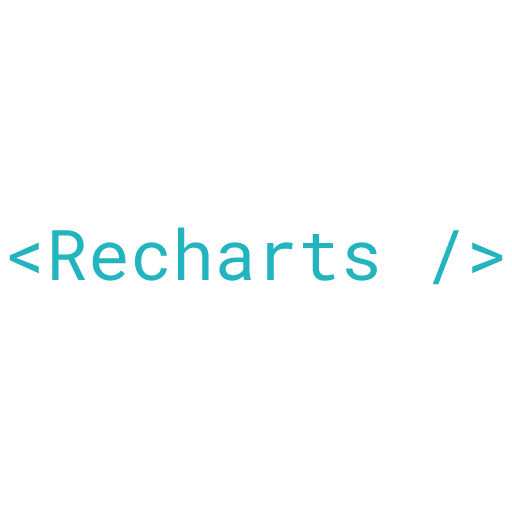
\includegraphics[width=\linewidth]{projet/images/recharts.png}
    \end{minipage}
    \hspace{1cm}
    \begin{minipage}[c]{0.6\textwidth}
        \textbf{Recharts.Js.}\\[0.5em]
    Est Une bibliothèque de graphiques composables construite sur des composants React.Créez rapidement vos graphiques avec des composants React découplés et réutilisables. \cite{ref17}
    \end{minipage}
\end{figure}
\vspace{0.5cm}

\begin{figure}[H]
    \centering
    \begin{minipage}[c]{0.3\textwidth}
        
\includegraphics[width=\linewidth]{projet/images/router-dom.png}
    \end{minipage}
    \hspace{1cm}
    \begin{minipage}[c]{0.6\textwidth}
        \textbf{React Router.}\\[0.5em]
    Est un package npm permettant d'implémenter le routage dynamique dans une application web. Il permet d'afficher des pages et de permettre aux utilisateurs de les parcourir. Il s'agit d'une bibliothèque de routage complète côté client et serveur pour React.  \cite{ref18}
    \end{minipage}
\end{figure}
\vspace{0.5cm}

\begin{figure}[H]
    \centering
    \begin{minipage}[c]{0.3\textwidth}
        
\includegraphics[width=\linewidth]{projet/images/Axios.png}
    \end{minipage}
    \hspace{1cm}
    \begin{minipage}[c]{0.6\textwidth}
        \textbf{Axios.}\\[0.5em]
   Axios, client HTTP basé sur les promesses, fonctionne de manière identique dans node.js et les navigateurs. \cite{ref19}
    \end{minipage}
\end{figure}
\vspace{0.5cm}

\begin{figure}[H]
    \centering
    \begin{minipage}[c]{0.3\textwidth}
        
\includegraphics[width=\linewidth]{projet/images/TanStack Query.png}
    \end{minipage}
    \hspace{1cm}
    \begin{minipage}[c]{0.6\textwidth}
        \textbf{TanStack Query.}\\[0.5em]
    Est une bibliothèque de gestion de l'état du serveur dans les applications React, permettant une gestion efficace des données asynchrones comme les requêtes API. \cite{ref20}
    \end{minipage}
\end{figure}
\vspace{0.5cm}

\begin{figure}[H]
    \centering
    \begin{minipage}[c]{0.3\textwidth}
        
\includegraphics[width=\linewidth]{projet/images/material-ui-.png}
    \end{minipage}
    \hspace{1cm}
    \begin{minipage}[c]{0.6\textwidth}
        \textbf{Material-ui.}\\[0.5em]
    Est une bibliothèque de composants React open-source qui met en
œuvre le design Material de Google. Il est complet et peut être utilisé dans la production à partir du carton. \cite{ref21}
    \end{minipage}
\end{figure}
\vspace{0.5cm}

\begin{figure}[H]
    \centering
    \begin{minipage}[c]{0.3\textwidth}
        
\includegraphics[width=\linewidth]{projet/images/lucide-react.png}
    \end{minipage}
    \hspace{1cm}
    \begin{minipage}[c]{0.6\textwidth}
        \textbf{lucide-react.}\\[0.5em]
    Est  une bibliothèque d'icônes open source proposant plus de 1 000 fichiers vectoriels (SVG) pour l'affichage d'icônes et de symboles dans des projets numériques et non numériques. \cite{ref22}
    \end{minipage}
\end{figure}
\vspace{0.5cm}
\begin{figure}[H]
    \centering
    \begin{minipage}[c]{0.3\textwidth}
        
\includegraphics[width=\linewidth]{projet/images/jwt.png}
    \end{minipage}
    \hspace{1cm}
    \begin{minipage}[c]{0.6\textwidth}
        \textbf{JSON Web Token.}\\[0.5em]
    Est un standard ouvert qui permet une échange sécurisé de tokens entre différentes parties. La sécurité de l’échange
se traduit par la vérification de l’intégrité et de l’authenticité des don-
nées. \cite{ref23}
    \end{minipage}
\end{figure}
\vspace{0.5cm}
\begin{figure}[H]
    \centering
    \begin{minipage}[c]{0.3\textwidth}
        
\includegraphics[width=\linewidth]{projet/images/AOS.png}
    \end{minipage}
    \hspace{1cm}
    \begin{minipage}[c]{0.6\textwidth}
        \textbf{AOS Animate On Scroll.}\\[0.5em]
    Est une bibliothèque open source d'animation par défilement créée par Michał Sajnóg . Elle a été créée pour optimiser les performances en utilisant uniquement du CSS pour les animations et en réservant JavaScript à la gestion de la logique. \cite{ref25}
    \end{minipage}
\end{figure}
\vspace{0.5cm}
\begin{figure}[H]
    \centering
    \begin{minipage}[c]{0.3\textwidth}
        
\includegraphics[width=\linewidth]{projet/images/toast.png}
    \end{minipage}
    \hspace{1cm}
    \begin{minipage}[c]{0.6\textwidth}
        \textbf{React-hot-toast .}\\[0.5em]
    Est une bibliothèque de notifications légère et open source pour React. Comme les autres bibliothèques React Toast, elle est conçue pour imiter les notifications push popularisées par les systèmes d'exploitation natifs, tels qu'iOS et Android, dans les applications web \cite{ref26}
    \end{minipage}
\end{figure}
\section{Architecture adoptée}
\subsection{Architecture logique :}
Avant d’entamer la conception et le développement de tout système informatisé, il est primordial d’élaborer son architecture.  Dans le cadre de notre projet,
nous avons choisi MVC (modèle-Vue-Contrôleur) en tant que patron d’architecture logicielle. Ce dernier permet d’organiser globalement une interface
graphique. En d’autres termes il permet de bien séparer le code de l’interface
graphique de la logique applicative D’ailleurs, c’est un choix populaire pour la
conception d’application web. En général ce modèle permet de distinguer trois
entités qui sont :
\begin{figure}[H]
    \centering
    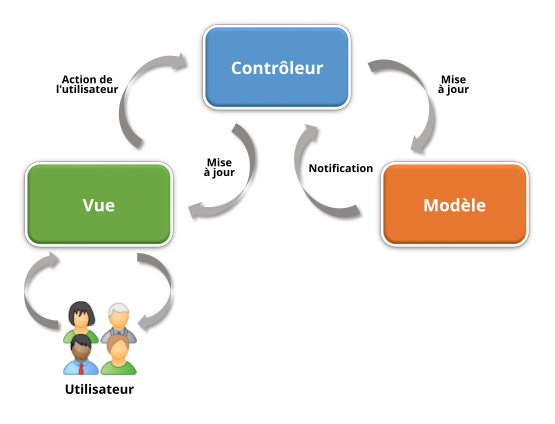
\includegraphics[width=0.6\linewidth]{projet/images/Model-View-Controller.png}
    \caption{L’architecture de Model-View-Controller}
    \label{fig:equipe_scrum}
\end{figure}

\textbf{• Modèle :}\\
contient les données manipulées par le programme. En effet il peut s’agir
d’un ensemble de fonctions (Modèle procédural) ou de classes (Modèle
orienté objet).\\
\textbf{• Vue :}\\
Fait l’interface avec l’utilisateur puisque elle donne plusieurs vues, elle
peut aussi présenter la possibilité à l’utilisateur de changer de vue.\\
\textbf{• Contrôleur :}\\
Un contrôleur contient la logique concernant les actions effectuées par
l’utilisateur.

\subsection{Architecture physique}
Pour assurer de bonnes performances, nous avons choisi une architecture
\textbf{client-serveur}.

Cette architecture est illustrée dans le schéma ci-dessous :

\begin{figure}[H]
    \centering
    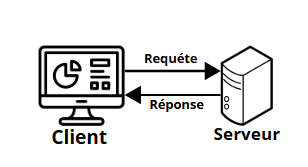
\includegraphics[width=0.6\linewidth]{projet/images/client-serveur.png}
    \caption{L’architecture client-serveur}
    \label{fig:equipe_scrum}
\end{figure}

\begin{itemize}
    \item \textbf{Le client} : que ce soit actif ou bien esclave, il lance la communication avec le serveur en adressant des demandes ou des requêtes.
    \item \textbf{Le serveur} : considéré comme passif ou maître, il répond aux demandes du client.
\end{itemize}

Grâce à cette séparation, chaque partie peut effectuer son travail de manière efficace et améliorer le système.
et plus organisé\\
\section*{Conclution}
Dans ce chapitre, nous avons présenté la planification de notre travail Alors
nous avons dégagé le premier artéfact le backlog de produit qui comporte les tous les liste des fonctionnalités de notre système, Par la suite nous avons dégagé ainsi les différents rôles de l’équipe dans le projet. Enfin nous avons choisi le concept de découpage pour la réalisation des sprints qui vont suivre, Nous allons enchainer à présent avec notre premier sprint dans le
chapitre qui suit.